\subsection{Execution}

\begin{frame}{Test case execution}{~}


\begin{minipage}{0.4 \textwidth}
    \begin{itemize}
    \setlength\itemsep{1em}
    \item system call traces and kernel stack traces are collected
    \item comapre sysetm call trees as AST
    \item limited to predictable systemcalls
\end{itemize}
\end{minipage}
\begin{minipage}{0.45\textwidth}
    \begin{figure}
        \center
    \def\stackalignment{l}
    \stackunder{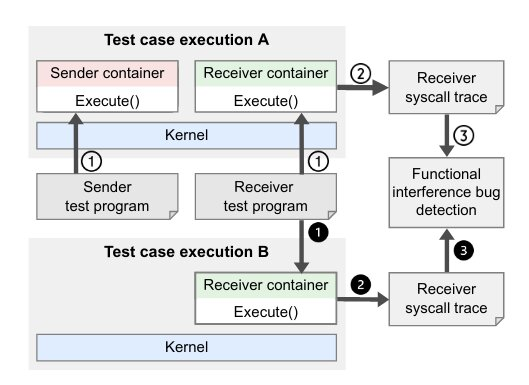
\includegraphics[scale=0.45]{/tmp/functionalInterferenceTesting}}
               {\scriptsize
                Source: C. Liu,S. Gong and P. fonseca, "KIT Testing }
                 {\scriptsize OS-Level Virtualization for Functional InterferenceBugs"(ASPLOS'23)}
    \end{figure}
            \end{minipage}


\end{frame}